\chapter{O arcabouço StarVZ} \label{ch:starvz}

Este Capítulo descreve em detalhes o arcabouço StarVZ. Este é 
apresentado genericamente na Seção \ref{sect:starvz-overview}, a Seção 
\ref{sect:starvz-phases} apresenta de forma detalhada as fases de sua 
execução, a Seção \ref{sect:related-work} disserta sobre otimizações já 
propostas e testadas e a Seção \ref{sect:motivation} fala sobre a motivação e a 
abordagem adotadas neste trabalho.

\section{Visão Geral}\label{sect:starvz-overview}

O StarVZ \cite{ref:starvz} é um fluxo de processamento de análise de desempenho 
cujo objetivo é auxiliar na avaliação e na verificação de hipóteses sobre a 
execução de aplicações baseadas em tarefas em ambientes heterogêneos, executados 
sobre o ambiente de execução StarPU \cite{ref:starpu}. Dentre as ferramentas de 
visualização de rastros desse tipo de aplicação, na pesquisa realizada foi 
identificado que o StarVZ se destaca pela utilização de ferramentas de 
Ciência de Dados para análise de desempenho.

Construído com uma abordagem de script, ele possui grande poder de customização. 
No trabalho de \citet{ref:starvz}, pode-se visualizar diversos gráficos de 
execução da aplicação: gráfico com comportamento de tarefas; gráfico com a 
quantidade de tarefas submetidas; o comportamento do ambiente de execução, com 
os estados dos trabalhadores StarPU; quantidade de tarefas prontas; 
taxa de GFlops (Gigaflops) do ambiente; tráfego de dados entre a memória das 
GPUs; transferências de rede MPI; e o número de operações MPI concorrentes.

Ele é composto de duas fases, que podem ser visualizadas de forma simplificada 
na Figura \ref{fig:starvz-workflow-general}.Cada uma delas é formada por uma 
combinação de diversas ferramentas, resultando em um arcabouço rápido, 
consistente, flexível e versátil.

\begin{figure}[H]
 \centerline{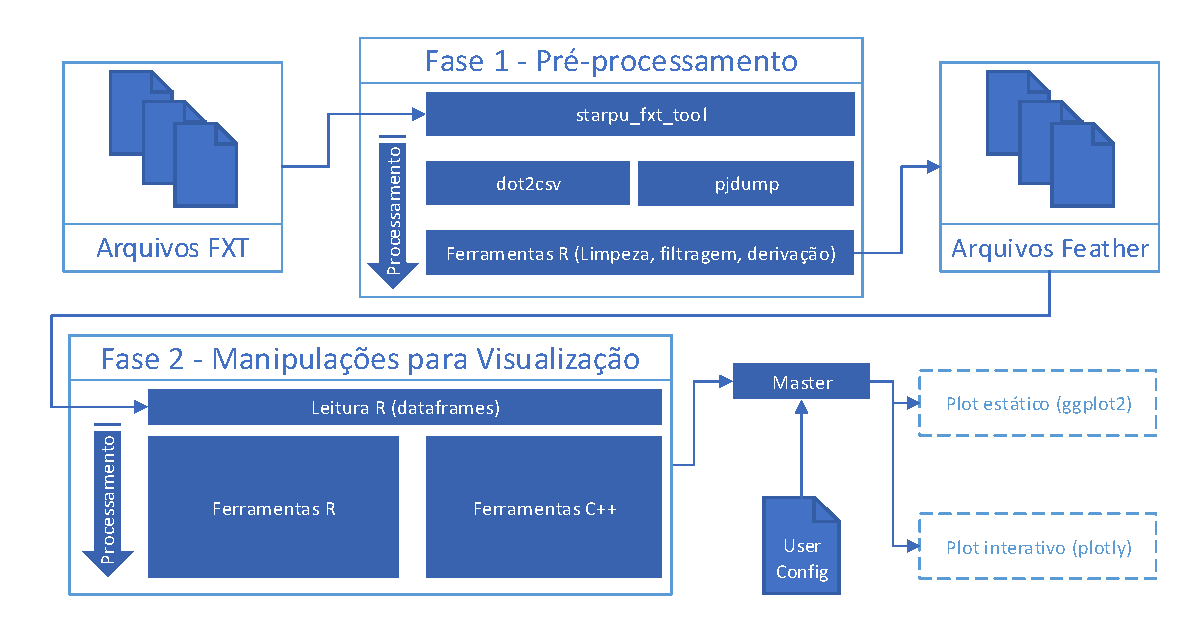
\includegraphics[width=1\textwidth]{./img/all-proc.pdf}}
 \caption{Fluxo de processamento do StarVZ.}
 \label{fig:starvz-workflow-general}
\end{figure}

\section{Fases}\label{sect:starvz-phases}

Na primeira fase, que pode ser visualizada na Figura \ref{fig:starvz-workflow1}, 
os rastros de execução do StarPU, que são arquivos no formato binário FXT, são 
transformados e exportados através da ferramenta \texttt{starpu\_fxt\_tool} para 
dois arquivos: DAG no formato DOT e Trace no formato PAJÉ. Essa etapa gera 
eventos datados, que descrevem o comportamento da aplicação para todos os 
recursos envolvidos. Também são gerados dados sobre o ambiente de execução do 
StarPU, como número de tarefas submetidas, número de tarefas prontas, 
arquitetura da plataforma, etc.

\begin{figure}[ht]
 \centerline{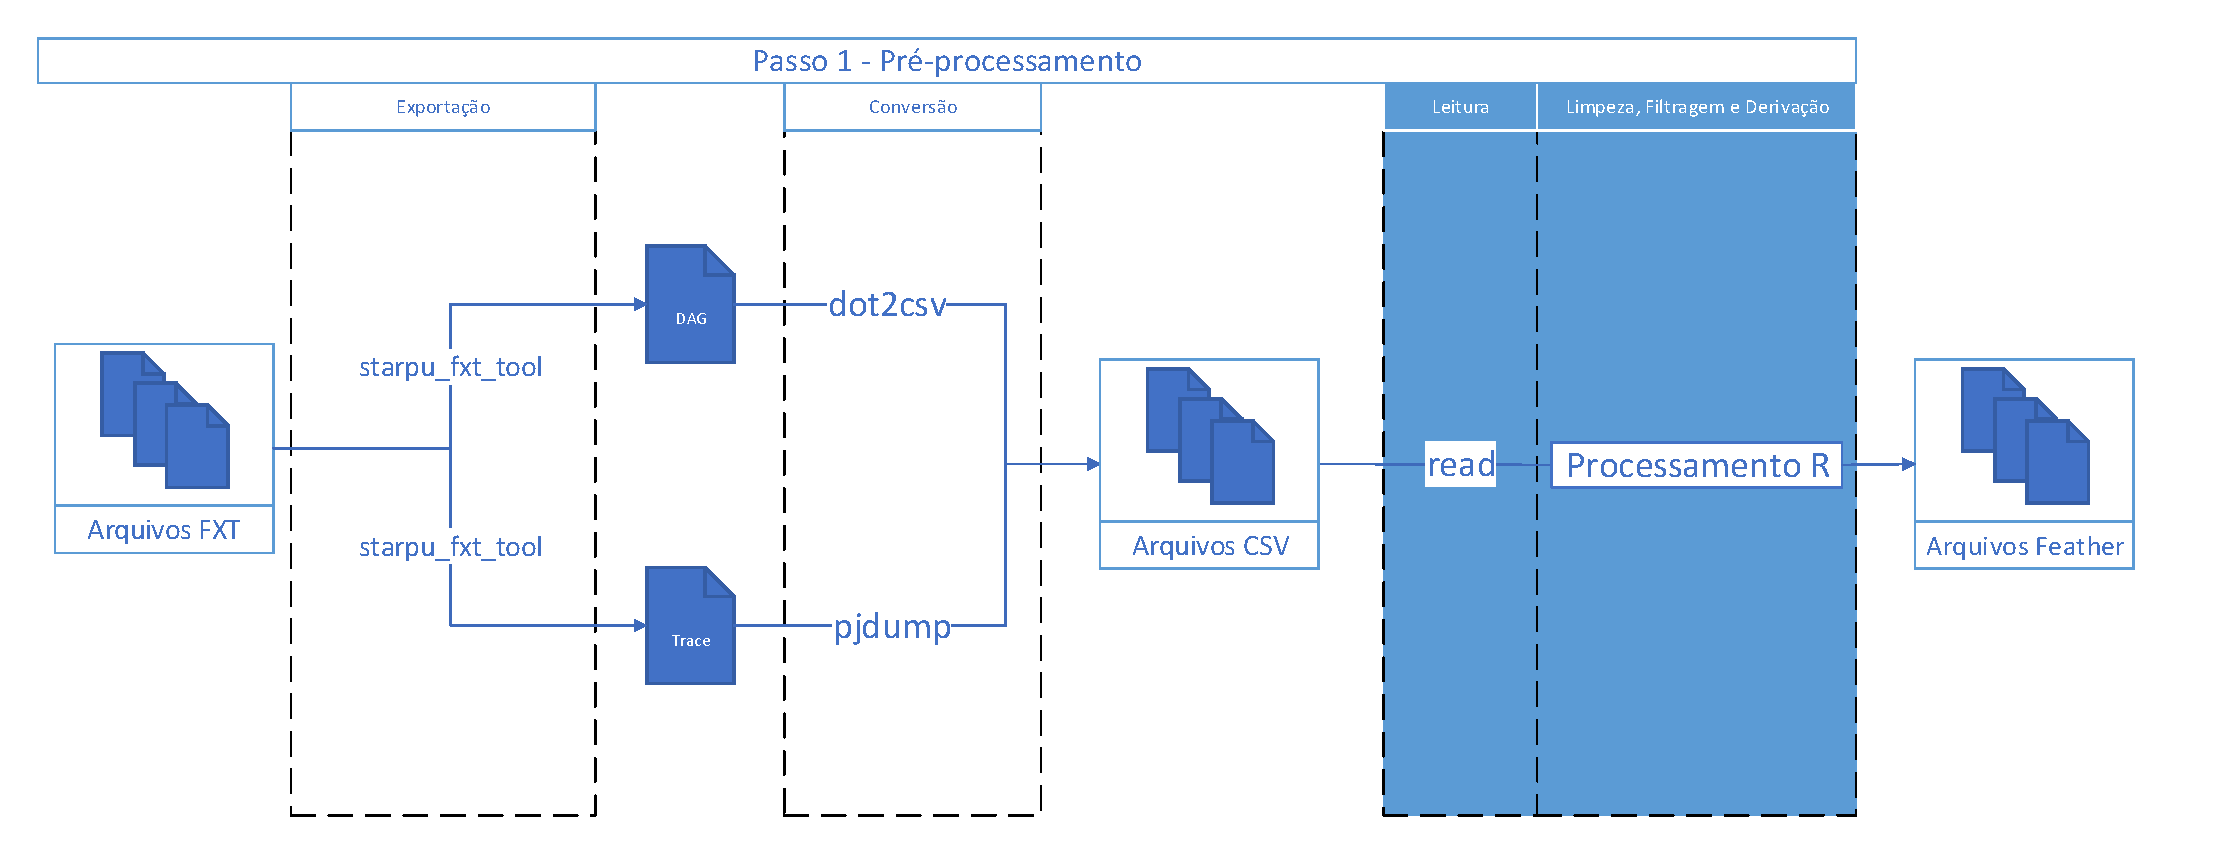
\includegraphics[width=1\textwidth]{./img/step1-simpler.pdf}}
 \caption{Fluxo de pré-processamento do StarVZ.}
 \label{fig:starvz-workflow1}
\end{figure}

Em seguida, é realizada uma verificação de integridade estrutural e temporal dos
arquivos \texttt{trace}. Ela é executada via \texttt{pj\_dump}, gerando cinco 
arquivos: o arquivo \textit{states} possui informações sobre as tarefas 
executadas e seu  comportamento no ambiente de execução; \textit{variables}
consiste em métricas de desempenho da plataforma e ambiente de execução; 
\textit{events} possui informações sobre a utilização de recursos; 
\textit{links} contém dados sobre comunicação MPI; e as informações de 
plataforma são registradas no arquivo \textit{entities}. O DAG também passa por 
uma conversão e por fim, todos os arquivos são gravados no formato de Valores 
Separados por Vírgula (\textit{Comma-Separated Value}, comumente abreviado para 
CSV).

Finalmente, os dados escritos em CSV são lidos, filtrados, agregados e 
combinados em uma ferramenta implementada na linguagem R, utilizando-se 
bibliotecas oriundas do pacote \texttt{tidyverse} para a manipulação de dados. 
As saídas são escritas no formato \textit{Feather} \cite{ref:feather}.

A segunda fase do fluxo de processamento inicia pela leitura das saídas da 
anterior. Cada arquivo torna-se uma tabela, e os dados são unificados em uma 
lista. É possível ter múltiplos rastros de aplicações sendo analisados em 
paralelo para comparação, basta multiplicar a leitura com entradas diferentes e 
elas podem posteriormente ser combinadas em uma única visualização. A criação 
dos gráficos ainda possui processamento de dados, o que traz certa flexibilidade 
para as visualizações. Como última etapa dessa fase, o usuário parametriza o 
sistema com um arquivo de configuração no formato YAML, para que a montagem da 
visualização seja configurável. Finalmente, o usuário pode analisar os gráficos 
gerados pela ferramenta.

Nos experimentos realizados em \citet{ref:starvz}, em uma máquina equipada com 
um Intel(R) Xeon(R) CPU E3-1225 v3 @3.20GHz e 32GB de memória principal e com 
uma entrada de aproximadamente 18GB, a primeira fase do fluxo de processamento 
levou cerca de 32 minutos para executar. A segunda fase, para executar a leitura 
dos arquivos \textit{Feather} e gerar a visualização levou em torno de 2 
minutos.

\section{Trabalhos Relacionados}\label{sect:related-work}

O trabalho de \citet{ref:drakestarvz} foi o primeiro a tentar otimizar o fluxo 
do StarVZ. Sua principal motivação foi a melhoria de desempenho da etapa de 
manipulação de dados, a mais custosa de acordo com os experimentos observados, 
com o objetivo de permitir o processamento de entradas maiores em um tempo 
aceitável. Nele utilizou-se \texttt{Drake} \cite{ref:drake}, uma biblioteca 
para a linguagem de programação R, cujo foco é executar apenas as 
partes necessárias de um fluxo de processamento de análise de dados, evitando 
os passos desnecessários que não mudarão suas saídas. Isso é realizado 
modelando as computações como um Grafo Acíclico Direcionado (\textit{directed 
acyclic graph} ou DAG) de tarefas e armazenando em cache os resultados daquelas 
já executadas. Além disso, \texttt{Drake} também possui suporte a paralelismo 
(\textit{Implicit parallelism}) para a execução de tarefas independentes.

Para modelar o StarVZ dessa forma, foram necessárias mudanças cujo objetivo era 
explicitar dependências e postergar junções de tabelas. Depois da identificação 
dos fluxos independentes no fluxo de processamento, foi utilizado \texttt{Drake} 
para criar um plano de execução, que consiste na declaração das tarefas onde 
cada uma é representada por uma função R. Na criação do plano, a biblioteca 
analisa cada uma das tarefas, suas entradas e saídas, para determinar 
dependências e gerar o DAG. O resultado da modelagem do StarVZ nessa abordagem 
pode ser visualizado na Figura \ref{fig:starvz-dag}.

\begin{figure}[ht]
\centerline{
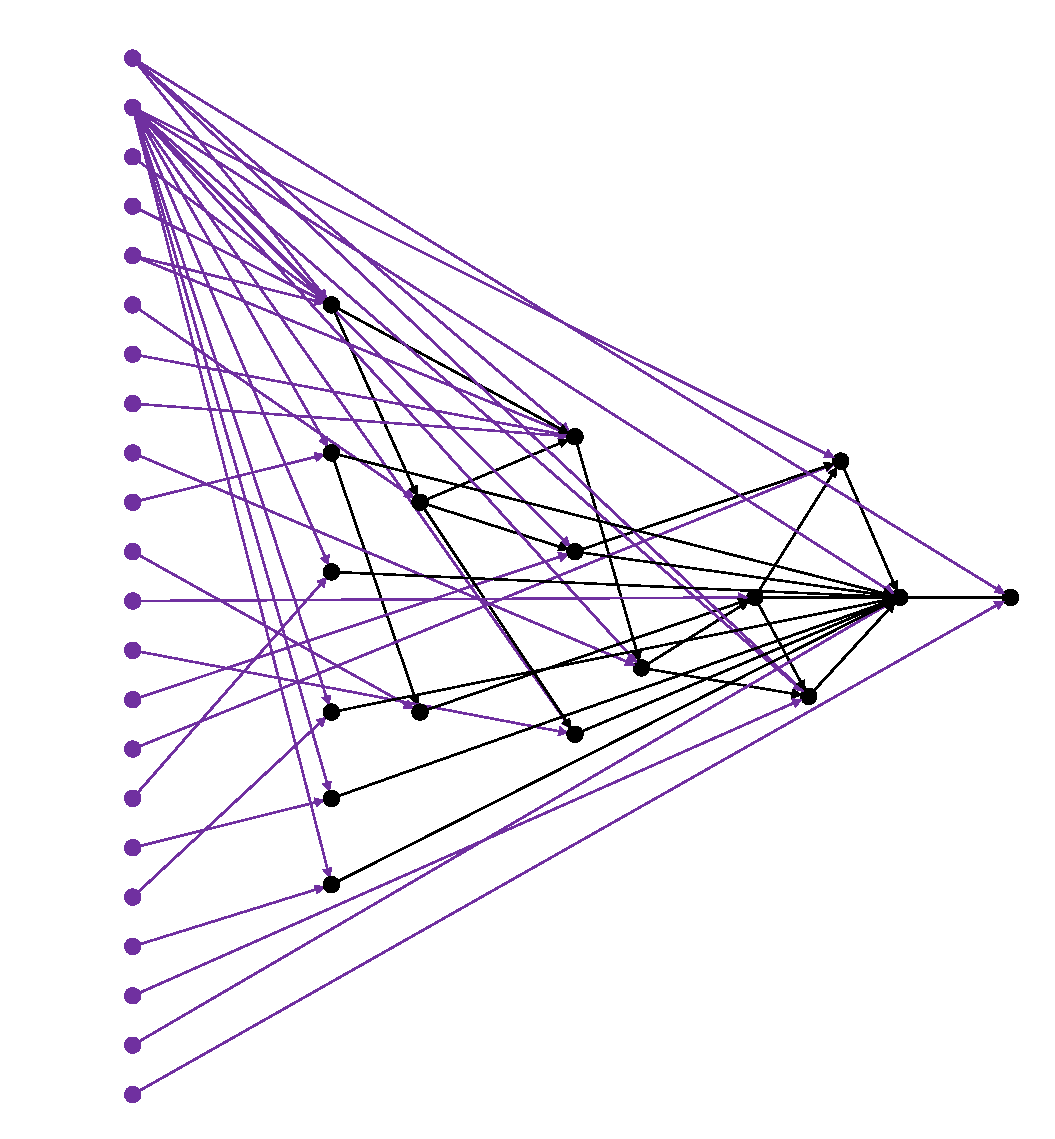
\includegraphics[width=0.8\textwidth]{./img/drake-dag-final-origin.pdf}}
 \caption{DAG de execução do StarVZ.}
 \legend{Fonte: Inspirada na Figura de contida no trabalho de 
\citet{ref:drakestarvz}}
 \label{fig:starvz-dag}
\end{figure}

Com esta modelagem, não foram observadas melhorias de desempenho no StarVZ. De 
acordo com \citet{ref:drakestarvz}, a cache de resultados intermediários da 
biblioteca acaba tendo que armazenar muitos dados em disco devido ao tamanho 
das tabelas geradas pelas entradas, prejudicando o tempo total de processamento.
Em relação ao suporte a paralelismo, ele é limitado pela falta de suporte 
nativo a \textit{multithread} da linguagem R. Por isso, \texttt{Drake} oferece 
essa funcionalidade instanciando múltiplas sessões R, que são processos 
separados. A comunicação entre esses processos é realizada pelo mesmo sistema 
de cache citado anteriormente, consequentemente, resultando nos mesmos 
problemas.

Outra abordagem que poderia ser adotada para melhorar o desempenho do StarVZ 
seria distribuir os fluxos independentes do fluxo de processamento pois elas 
podem trazer um ganho de desempenho em um ambiente viável. Ao simplesmente 
paralelizar, é possível que os mesmo problemas com o tamanho das tabelas sejam 
enfrentados, exigindo máquinas com muita memória para obter-se os resultados 
desejados. 

A primeira opção seria distribuir os fluxos independentes utilizando o pacote 
\texttt{Snow}, que significa \textit{Simple Network of Workstations} 
\cite{ref:snow}. Este é desenvolvido para linguagem R e permite a utilização
de \textit{Explicit parallelism}, oferecendo integração com três interfaces de 
baixo nível: PVM (\textit{Parallel Virtual Machine}), através do pacote 
\mytexttt{rpvm}; MPI, através do pacote \mytexttt{rmpi} \cite{ref:rmpi}; e uma 
integração com sockets, no caso de não ter nenhuma das outras opções disponíveis 
no ambiente. A utilização de \mytexttt{Snow} pode ser feita através da 
biblioteca \texttt{Snowfall} \cite{ref:snowfall}, que é uma camada cujo objetivo 
é melhorar a usabilidade, 
facilitando ainda mais a utilização.

A segunda alternativa seria a utilização da biblioteca \texttt{future} 
\cite{ref:future}. Esta provê uma forma simples e uniforme de avaliar expressões 
de forma assíncrona, utilizando recursos diversos. Ela funciona utilizando o 
conceito de abstração \textit{future}, que basicamente define um valor que 
poderá 
estar disponível no futuro. Tal valor pode ter seu estado como resolvido ou não 
resolvido, estado em que se ele for utilizado bloqueará o processo até sua 
resolução. Os \textit{futures} podem ser resolvidos de diversas formas: 
sequential, onde são resolvidos sequencialmente no processo R corrente; 
multiprocess, que resolve utilizando \textit{multicore}; cluster, que é o mais 
interessante para adoção pois resolve com sessões R na máquina local e/ou em 
máquinas remotas; e etc.

\section{Motivação e Abordagem}\label{sect:motivation}

Há algum tempo, vivemos na era dos dados. O volume armazenado em meios 
eletrônicos é difícil de medir, mas existem alguns estudos que podem nos 
auxiliar a ter uma noção disso. A IDC (\textit{International Data Corporation}) 
\cite{ref:idcdigitaluniverse} estima que, de acordo com o histórico de 
crescimento do mundo digital, este deve crescer entre 2013 e 2020 de 4.4 para 44 
zettabytes \footnote{Um zettabyte significa um trilhão de gigabytes.}.

Conforme explicitado na Seção \ref{sect:starvz-phases}, o tempo total de 
execução da primeira Fase do StarVZ, para uma carga de trabalho de 18 gigabytes 
levou cerca de 32 minutos. Para viabilizar o processamento de maiores volumes de 
dados em um tempo aceitável, trazendo as vantagens da utilização da ferramenta 
para esses cenários, é necessário otimizar esta Fase do fluxo de processamento.

Decompondo esse tempo entre todas as ferramentas utilizadas, a Tabela 
\ref{tab:exectimes} exibe o tempo de cada ferramenta no fluxo de processamento 
para a execução mencionada no trabalho de \citet{ref:starvz}. Como o volume de 
dados utilizado foram apenas 18 gigabytes, essas aplicações não possuem um tempo 
de execução razoável para tratamento de grandes volumes de dados.

\begin{table}[H]
\centering
\small
\begin{tabular}{l c c} \toprule
\textbf{Ferramenta}  &  \textbf{Tempo de Execução}  & \textbf{Tempo Relativo}\\ \midrule
starpu\_fxt\_tool     & 10 minutos   & 31,25\%  \\
pj\_dump            & 9 minutos    & 28,12\%     \\
Ferramenta R        & 13 minutos   & 40,62\%      \\
\textbf{Total}     & 32 minutos & -
\end{tabular}
\caption{Arcabouço StarVZ - Tempos de execução da primeira Fase.}
\label{tab:exectimes}
\end{table}

Como na segunda fase não é evidente um ponto de otimização urgente, tendo em 
vista que nos experimentos foram gerados resultados em poucos minutos, a 
motivação deste trabalho é a otimização do ponto mais crítico do tempo de 
execução da primeira fase do fluxo de processamento. Como as ferramentas 
desenvolvidas em R manipulam tabelas, fazendo operações comuns a Ciência de 
Dados, este trabalho migrará as tabelas normais para tabelas Spark, com o 
intuito de distribuir o trabalho em diversas máquinas. Além disso, para esta 
adaptação suportar arquivos muito grandes, essa instância do Spark irá
executar sobre o Hadoop, garantindo que os dados terão uma manipulação 
otimizada.